\section{System Architecture}
\begin{figure}[H]
\centering
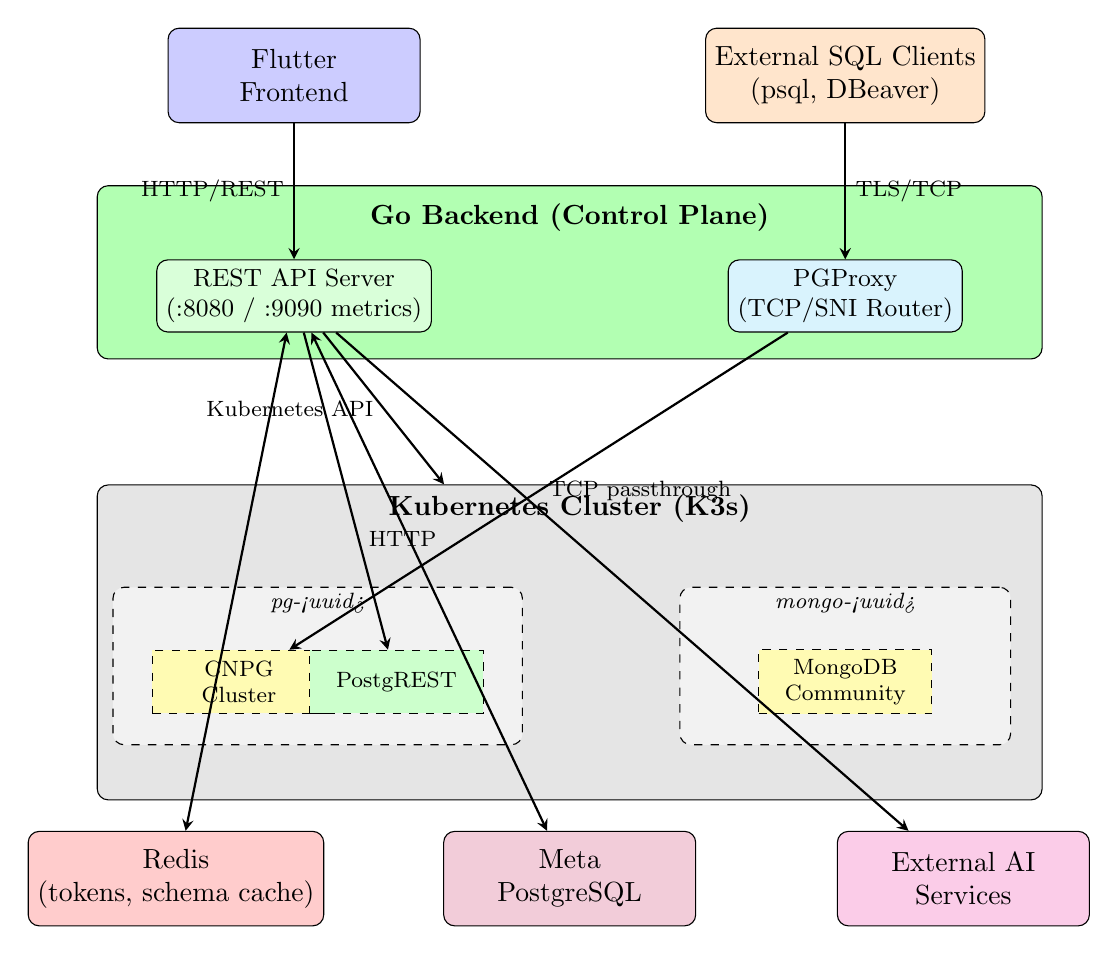
\begin{tikzpicture}[
    box/.style={rectangle, draw, minimum width=3.2cm, minimum height=1.2cm, align=center, rounded corners},
    smallbox/.style={rectangle, draw, minimum width=2.6cm, minimum height=0.9cm, align=center, rounded corners, font=\small},
    container/.style={rectangle, draw, dashed, minimum width=2.2cm, minimum height=0.8cm, align=center, font=\footnotesize},
    arrow/.style={->, thick, >=stealth},
    darrow/.style={<->, thick, >=stealth}
]
    % Client Layer
    \node[box, fill=blue!20] (flutter) at (-3.5,7) {Flutter\\Frontend};
    \node[box, fill=orange!20] (sqlclient) at (3.5,7) {External SQL Clients\\(psql, DBeaver)};

    % Control-plane processes (two binaries, one image)
    \node[box, fill=green!30, minimum width=12cm, minimum height=2.2cm] (backend) at (0,4.5) {};
    \node at (0,5.2) {\textbf{Go Backend (Control Plane)}};

    \node[smallbox, fill=green!15] (api) at (-3.5,4.2) {REST API Server\\(:8080 / :9090 metrics)};
    \node[smallbox, fill=cyan!15] (pgproxy) at (3.5,4.2) {PGProxy\\(TCP/SNI Router)};

    % K8s Cluster Layer
    \node[box, fill=gray!20, minimum width=12cm, minimum height=4cm] (k8scluster) at (0,-0.2) {};
    \node at (0,1.5) {\textbf{Kubernetes Cluster (K3s)}};

    % PostgreSQL project namespace
    \node[box, fill=gray!10, dashed, minimum width=5.2cm, minimum height=2cm] (pgns) at (-3.2,-0.5) {};
    \node at (-3.2,0.3) {\footnotesize \textit{pg-<uuid>}};
    \node[container, fill=yellow!30] (tenant1) at (-4.2,-0.7) {CNPG\\Cluster};
    \node[container, fill=green!20] (postgrest) at (-2.2,-0.7) {PostgREST};

    % MongoDB project namespace
    \node[box, fill=gray!10, dashed, minimum width=4.2cm, minimum height=2cm] (mongons) at (3.5,-0.5) {};
    \node at (3.5,0.3) {\footnotesize \textit{mongo-<uuid>}};
    \node[container, fill=yellow!30] (tenant2) at (3.5,-0.7) {MongoDB\\Community};

    % Platform services
    \node[box, fill=red!20] (redis) at (-5,-3.2) {Redis\\(tokens, schema cache)};
    \node[box, fill=purple!20] (platformdb) at (0,-3.2) {Meta\\PostgreSQL};
    \node[box, fill=magenta!20] (aiagent) at (5,-3.2) {External AI\\Services};

    % Arrows
    \draw[arrow] (flutter) -- (api) node[midway, left, font=\footnotesize] {HTTP/REST};
    \draw[arrow] (sqlclient) -- (pgproxy) node[midway, right, font=\footnotesize] {TLS/TCP};

    \draw[arrow] (api) -- (k8scluster) node[midway, left, font=\footnotesize] {Kubernetes API};
    \draw[arrow] (pgproxy) -- (tenant1) node[midway, right, font=\footnotesize] {TCP passthrough};
    \draw[arrow] (api) -- (postgrest) node[pos=0.65, right, font=\footnotesize] {HTTP};

    \draw[darrow] (api) -- (platformdb);
    \draw[darrow] (api) -- (redis);
    \draw[arrow] (api) -- (aiagent);
\end{tikzpicture}
\caption{High-Level System Architecture}
\label{fig:architecture}
\end{figure}

\begin{itemize}
    \item \textbf{Decoupled Control-Plane Processes:} The backend ships as one Docker image containing two binaries---the REST API server and a dedicated \texttt{pgproxy} process for PostgreSQL TCP routing. They deploy as separate Kubernetes workloads but share the same codebase and release artifact.
    \item \textbf{Kubernetes Operator Pattern:} Tenant databases are managed via custom resources (CRDs), enabling declarative lifecycle management and operator-driven reconciliation.
    \item \textbf{Per-Project Namespace Isolation:} Each provisioned project receives its own Kubernetes namespace (\texttt{pg-<uuid>} for PostgreSQL or \texttt{mongo-<uuid>} for MongoDB), enclosing the database cluster, Secrets, Services, and engine-specific sidecars such as PostgREST.
\end{itemize}
